\section{Results}%
\label{sec:Results}

\begin{figure}[p]
    \centering
    \begin{subfigure}{0.45\textwidth}
        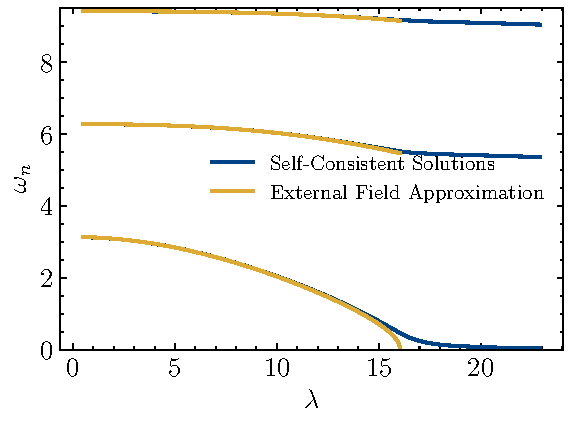
\includegraphics[width=\textwidth]{Figures/dirichlet/eigenvalues.pdf}
    \end{subfigure}
    \begin{subfigure}{0.45\textwidth}
        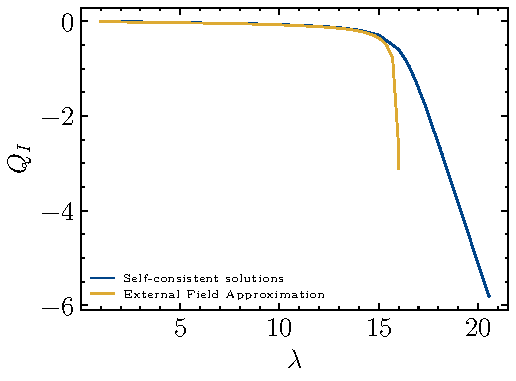
\includegraphics[width=\textwidth]{Figures/dirichlet/inducedCharge.pdf}
    \end{subfigure}
    \begin{subfigure}{0.45\textwidth}
        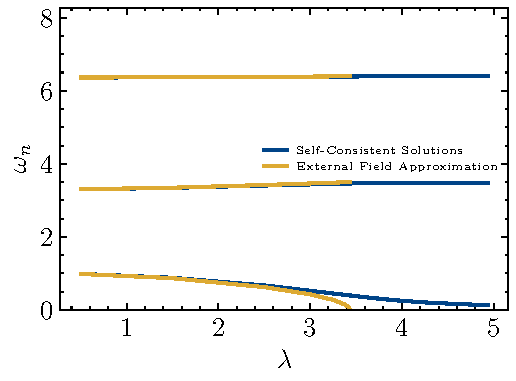
\includegraphics[width=\textwidth]{Figures/neumann/eigenvalues.pdf}
    \end{subfigure}
    \begin{subfigure}{0.45\textwidth}
        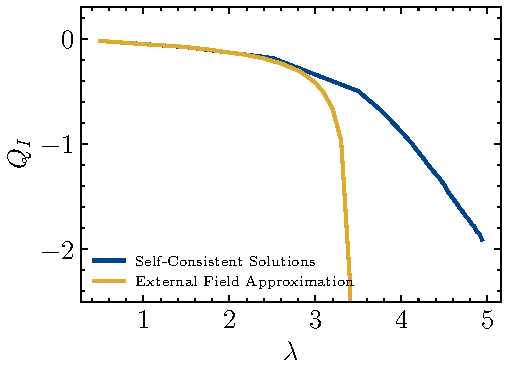
\includegraphics[width=\textwidth]{Figures/neumann/inducedCharge.pdf}
    \end{subfigure}
    \caption{Top left panel: Energy of the three first modes of the massless
    Klein-Gordon field with Dirichlet boundary conditions
    corresponding to different values of the dimensionless backgroud electric
    field strength $\lambda.$ In blue, the self-consistent mode energies
    $\omega_{n,\lambda}^{\infty}$. For reference, the energies of the lower
    modes in the External Field Approximation is shown. Top right panel:
    Corresponding induced charge $Q_I$ as a function of $\lambda$.
    Bottom left panel:
    Massive $(m=1)$ Klein-Gordon field with Neumann boundary conditions
    corresponding to different values of the dimensionless backgroud
    electric field strength $\lambda.$ In blue, the energies
    $\omega_{n,\lambda}^{\infty}$ of the self-consistent solutions to the
    Klein-Gordon-Maxwell equations. Bottom right panel: The induced charge for
    said configuration.
}
    \label{fig:self-consistent-eigenvalues}
\end{figure}

We use the iterative procedure laid out in  
Sec.~\ref{sec:The-iterative-procedure} to study the interaction between the
scalar field and the background electric field for two particular cases, $m=0$
with the scalar field subject to Dirichlet boundary conditions, and $m=1$ with
the scalar field subject to Neumann boundary conditions, as there are no
massless solutions to the Klein-Gordon equation with Neumann boundary
conditions.

Fig.~\ref{fig:self-consistent-eigenvalues} displays the evolution of the
self-consistent mode energies of the mentioned cases as described in the
caption in blue, and compares it with the external field approximation, in
orange. Following a similar format, the self-consistent induced charge $Q_I$ is
shown, and in orange the reference for the external field approximation.

Notice the almost identical behavior of the self-consistent solutions to the
external field approximation for $\lambda \ll {\lambda_c}$ in both cases. For
$\lambda \gtrsim \lambda_c$, the inclusion of backreaction raises the energy of
the Klein-Gordon field and avoids the instabilities ($\omega_n \to 0$, $\lvert
Q_I\rvert \to \infty$) that the external field approximation presented.

